\chapter{Discussion}\label{discussion}

This chapter reads the verdicts of §4 as a single account, returns to what the adversarial design contributed, then turns from the swarm to the questionnaire. It closes with the threats to the figures reported.

\section{The Scorecard}\label{the-scorecard}

The six criteria were introduced in §2.2 as the conditions under which an automated assessment stays contestable, and Chapter 4 returned a verdict on each. Read individually, those verdicts show multiple failure modes: abstention tracking maturity, correct negatives clustering below the confidence threshold, answer variance between runs. Read together, they describe a single constraint that affects everything downstream, data availability. This section works through the criteria in the order that makes that constraint visible, starting from the result most in need of explanation. The system reproduces the human process closely on the answers it commits to, yet when it is forced to answer every question its accuracy falls below what a fixed reply of yes would score. Its competence is therefore real but conditional on being allowed to decline, and what follows sets out what it is declining and why.

Convergent Validity establishes that there is agreement with the key, under certain conditions. On the pairs it commits to, the system agrees with the published key about seven times in ten, which is close reproduction of the existing process, but that figure holds only because it first sets aside almost half of the questions. The system recovers most of the positive answers and few of the negative ones, so the accuracy it reaches in normal operation is bought by declining the questions whose true answer is no. This locates the weakness exactly, and @@CL@@this is the optimism bias §2.3 anticipated@@/CL@@. It raises the question of why the system cannot commit a negative answer as reliably as a positive one.

Selectivity supplies the reason, and the reason is structural. The confidence score the system attaches to an answer measures how well the retrieved evidence supports the label it chose, and that quantity is not symmetric across the two labels. A positive answer can be evidenced directly, a negative answer has no equivalent, because the absence of a practice leaves nothing to quote. Confidence therefore tracks how easily a claim could be evidenced rather than how likely it is to hold, the asymmetry of Figure 4.2.2, and negative answers often sit under the commit threshold whatever their merit. The calibration results bear this out, with the system well behaved on positive golds and inverted on negative ones, most confident on the negatives at the point where it is most often wrong. The abstention seen under Convergent Validity is the system declining the answers it cannot evidence, which is the behaviour the criterion asks for, and it leaves the negative class structurally underserved.

Attributability removes the innocent reading of those errors, the possibility that the system is simply inventing them. The first of its two conditions, that a quoted passage exists in the retrieved text, is enforced mechanically before any answer commits, and every committed answer in the run satisfied it. Fabrication is therefore not the failure mode, and the positive answers the system commits are grounded in text it retrieved. What this leaves is more nuanced, because the wrong positives are drawn from real material that sits near the question. The system finds a relevant document, quotes a tangential passage, and reads it as proof. The second condition, that a reader would agree the passage supports the claim, is the one the Verifier set out to enforce, and it is where the remaining error lives.

Generalisability shows that this over-reading is not uniform but scales with how much adjacent material a question attracts. Where the evidence is dispositive the system is strong, and the portal dimension is the clearest case, since a portal feature is either present on the page or it is not and there is little room to over-read. Where the evidence is abundant without being decisive the system is weakest, and the policy dimension is the clearest case of that, since a draft strategy, an unadopted obligation or a regional initiative all resemble the national instrument a question asks about closely enough to be taken for it. Policy accordingly commits more readily than any other dimension and returns a wrong positive on half of its negative questions. This extends to the poor performance on all non-binary questions. The swarm declines almost everything that asks for a graded or computed figure, since those questions rarely offer a single passage that settles them.

Subgroup Equity carries the same mechanism from questions to countries. The stratification was built to detect a language effect, on the expectation that weaker comprehension of a national language would produce confident error, and that effect did not appear. What appeared instead is that measurement error tracks maturity. A mature country does most things, so a question whose true answer is no is still surrounded by adjacent evidence of related practices, and the open web returns abundant material that reads as support for yes. A less mature country more often lacks the practice outright, and the web returns little that could be mistaken for it. The false-positive rate consequently rises with a country\textquotesingle s published maturity while coverage falls as maturity falls, the two panels of @@CC@@Figure 5.1@@/CC@@, so a country\textquotesingle s assessed result depends in part on where it already sits on the scale the index exists to measure. An error that correlates with the quantity being estimated is a bias rather than noise, and the distinction matters for what follows, because noise averages out when many questions are pooled into a score and bias does not.

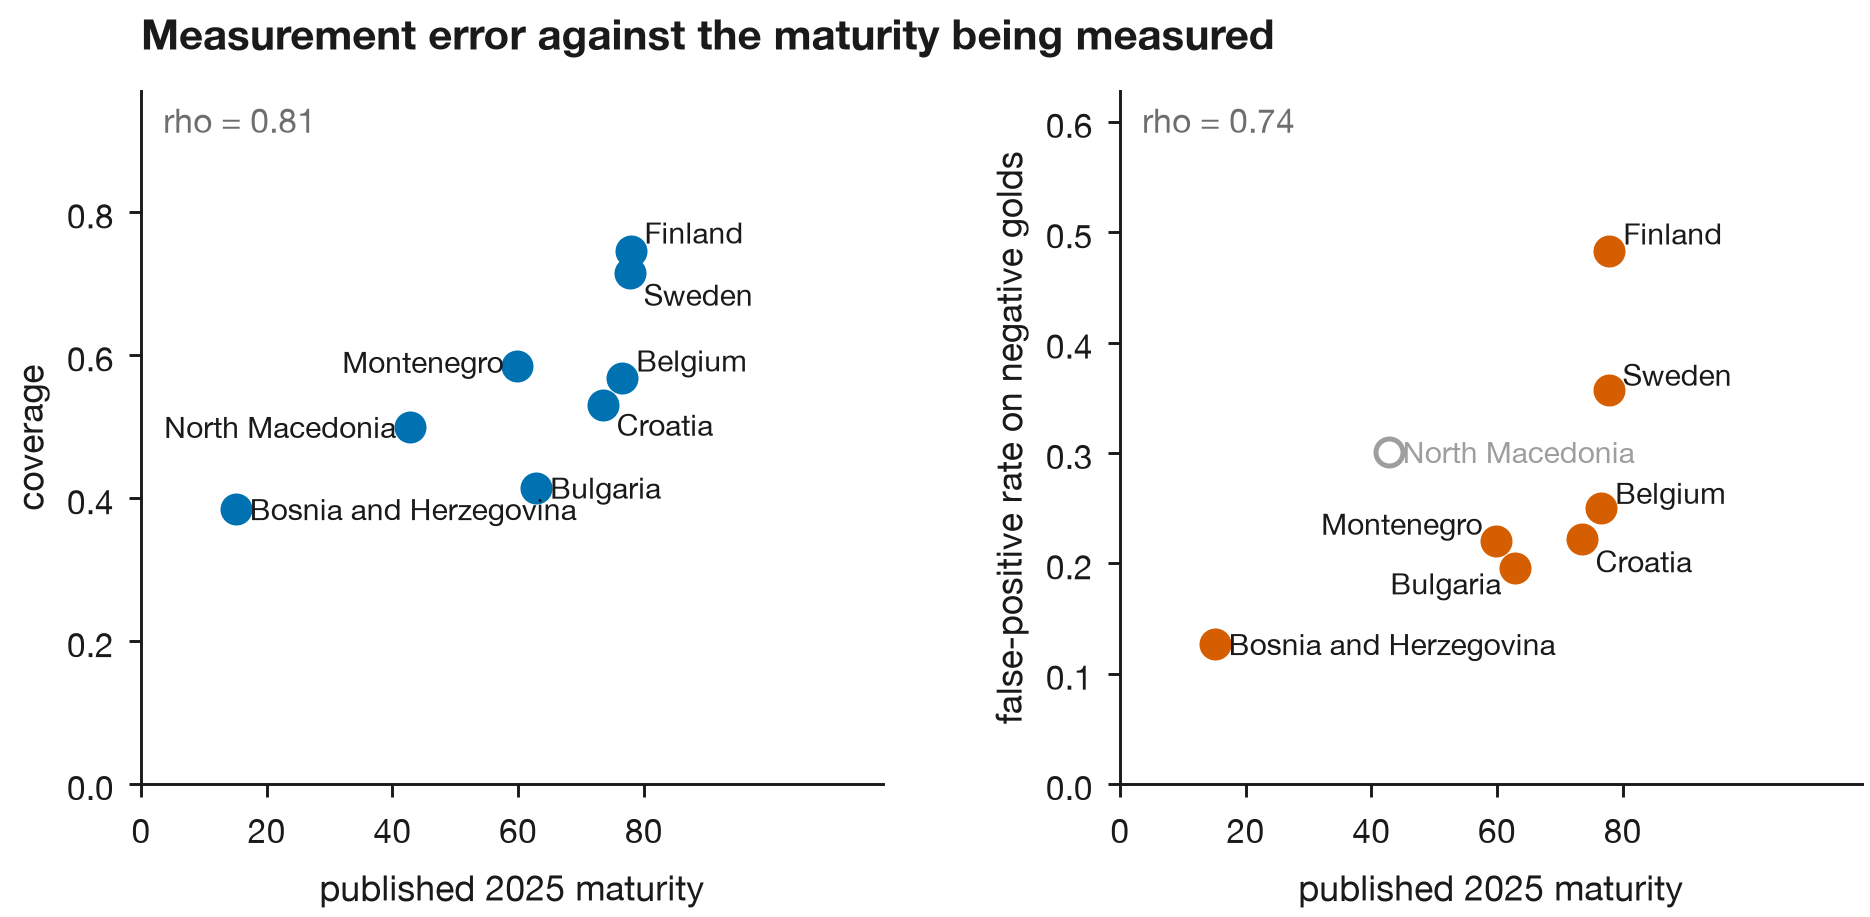
\includegraphics[width=5.9in,height=2.89321in]{media/media/image19.png}

@@CC@@Figure 5.1: Measurement error against the maturity being measured. North Macedonia, hollow, is the one country off the false-positive trend.@@/CC@@

Reproducibility confirms the same account from a third direction. Run three times over one battery with the search cache cleared between runs, the system reached the same outcome on around seven pairs in ten, and almost all of the disagreement concerned whether to answer rather than what to answer. When all three runs did commit they agreed on the label nearly every time, so the answer itself is stable and the instability sits in the decision to commit. That instability concentrates on the thin-evidence negatives whose confidence rests just above the threshold. The overall score is fairly stable, because a score pooling many questions absorbs the individual flips and commit-accuracy barely moves across the runs. The traceability condition is met for the headline run, whose logs allow every figure to be re-derived, so the part of the system that fails is judgement under thin evidence and not the discipline of the record.

Set end to end, the six verdicts@@CL@@ in Table 5.1@@/CL@@ describe one system. It is a competent retriever of positive evidence working in a setting where negative facts cannot be evidenced, and each criterion has shown a different face of this constraint. The grounded positives, the stable pooled score and the ruling-out of fabrication are what the constraint allows, while the below-baseline accuracy when forced to answer and the error that grows with the maturity being measured result from it.

@@CC@@RQ1 asked whether an automated assessment@@/CC@@ can meet the conditions that keep it legitimate, and the answer here is split. A country can see the evidence behind each answer and can see which of its questions the system declined, so the result is auditable in a way the closest comparable work is not. It cannot assume that a neighbouring country met the same standard, because the standard varies with the maturity being assessed. Automation can preserve transparency that makes an assessment challengeable, and a swarm architecture provides this where a single `black-box' agent @@CC@@cannot@@/CC@@. Yet, this does not yet preserve the even treatment that makes a ranking fair, and §5.3 sets out the change to the questionnaire that would remove that dependence.

{\def\LTcaptype{none} % do not increment counter
\begin{longtable}[]{@{}
  >{\raggedright\arraybackslash}p{(\linewidth - 8\tabcolsep) * \real{0.1635}}
  >{\raggedright\arraybackslash}p{(\linewidth - 8\tabcolsep) * \real{0.1641}}
  >{\raggedright\arraybackslash}p{(\linewidth - 8\tabcolsep) * \real{0.1111}}
  >{\raggedright\arraybackslash}p{(\linewidth - 8\tabcolsep) * \real{0.2806}}
  >{\raggedright\arraybackslash}p{(\linewidth - 8\tabcolsep) * \real{0.2806}}@{}}
\toprule\noalign{}
\begin{minipage}[b]{\linewidth}\raggedright
\textbf{Criterion}
\end{minipage} & \begin{minipage}[b]{\linewidth}\raggedright
\textbf{§2.2 condition}
\end{minipage} & \begin{minipage}[b]{\linewidth}\raggedright
\textbf{Verdict}
\end{minipage} & \begin{minipage}[b]{\linewidth}\raggedright
\textbf{Load-bearing evidence}
\end{minipage} & \begin{minipage}[b]{\linewidth}\raggedright
\textbf{Conclusion}
\end{minipage} \\
\midrule\noalign{}
\endhead
\bottomrule\noalign{}
\endlastfoot
\textbf{Convergent Validity} & Agreement with the ODMI key, and with a measure computed independently of it & Half met & Commit-accuracy 0.701 (437 of 623 scoreable committed) at coverage 0.556 (636 of 1,144). Scoring every abstention as an error, raw accuracy 0.424 (385 of 907 binary golds) against the 0.594 always-yes baseline, and balanced accuracy 0.396 against the 0.500 any single-class rule returns. Catalogue recompute against the published key, agreement on 18 of 32 measurable cells across four countries, so 44\% divergence & An automated assessment reproduces the human process on the answers it is willing to give, which is half the questionnaire. The recompute puts the answer key itself in doubt on the nine catalogue questions, so agreement with that key measures how closely the system tracks the existing process and leaves correctness open \\
\textbf{Selectivity} & Commits only where the evidence supports it, abstains otherwise, with a stated confidence that tracks observed accuracy & First condition met, second failed & Declines on 44.4\% (508 of 1,144). Aggregate ECE 0.063 over 623 scoreable committed answers, splitting to 0.089 on yes golds and 0.299 on no golds, where the sequence inverts. 86 of the 142 scoreable committed noes sit exactly at the 0.65 floor and none exceeds 0.90. Of the 88 withheld sub-floor answers carrying a no gold, 73 matched the key. & The abstention channel makes the output safe to publish, because a declined question reaches the country as a visible gap. The stated confidence carries no usable signal on the negative class, where it falls as correctness rises, so a country cannot read it as a measure of how far to trust an answer \\
\textbf{Attributability} & The quoted passage exists in the cited source, and a reasonable reader agrees it supports the claim & Settled one way, open the other & All 636 committed answers passed the offline gate, and 24 abstentions (4.7\% of 508) record an ungrounded passage against 208 (40.9\%) Verifier relevance rejections. Of the 94 negative-gold false positives, 0 of the 91 adjudicable cases vindicated the swarm & A country can contest any answer held against it, because every committed answer carries a passage present in the text the system retrieved. Whether that passage supports the label is unmeasured outside the swarm, and the false-positive audit puts the residual error there, in material that sits near the question without settling it \\
\textbf{Subgroup Equity} & Adequate performance within each subgroup, with results split by native language and maturity & Not met. The language leg came back clean and the maturity leg fails & Language leg, stratum A negative-gold false-positive rate 0.211 (55 of 261) against stratum B 0.336 (36 of 107), and committed-negative recall 0.272 against 0.178. Maturity leg, coverage, commit-accuracy and negative-gold false-positive rate all rise with published maturity at Spearman 0.81, 0.88 and 0.74 across the eight countries. Finland 0.483 (14 of 29) at maturity 77.9, Bosnia and Herzegovina 0.128 (10 of 78) at 15.1 & A ranking built from this system holds countries to different standards, because its error rises with the maturity it is trying to measure. Pooling more questions does not remove that, since an error correlated with the quantity being estimated behaves as bias and survives aggregation \\
\textbf{Generalisability} & Results decomposed by answer type and by ODMI dimension & Not met. Performance varies by dimension and collapses on the graded shapes & Commit-accuracy from 0.784 (145 of 185) on Portal to 0.622 (102 of 164) on Impact, and negative-gold false-positive rate from 0.132 (15 of 114) on Portal to 0.500 (33 of 66) on Policy. The four percentage-band questions with no catalogue route are declined on all 32 of their pairs, and the count-band questions return 1 exact match across 16 pairs. Graded questions are 19 of the 143, and 10 of 143 once the nine catalogue questions are set aside & The system can take a defined part of the questionnaire, since its accuracy follows how far the available evidence settles a question. Any published result would have to carry its per-dimension reliability, because a Policy pass and a Portal pass mean different things \\
\textbf{Reproducibility} & Traceability, a record complete enough to re-derive any reported figure. Stability, measured as variance between runs & Traceability met with one gap. Stability holds for the score and fails per question & Every Researcher, Verifier and Adjudicator call writes its prompt version, model version and raw response; the snippet picker writes no equivalent row, so its prompt and model version sit outside the record. Three replicates over the 148-pair development intersection, outcome unanimity 0.703, label agreement 0.922 (47 of 51) once all three commit, and commit-accuracy range 0.014 & The figure the ODMI would publish survives a repeat run, because the per-question flips offset each other once 143 questions pool into a score. A country reading a single answer gets a weaker guarantee, since whether the system answers that question at all moves between runs \\
\end{longtable}
}

@@CC@@Table 5.1: The six criteria of §2.2, and the verdict Chapter 4 returned on each.@@/CC@@

\section{Debate in an ODMI Environment}\label{debate-in-an-odmi-environment}

@@CC@@RQ2 asked what a swarm of distinct roles@@/CC@@ adds over a single agent, and what the adversarial stance adds in particular. The design\textquotesingle s premise was that an adversarial second agent would decorrelate the blind spots that produce an error, on the reasoning of Cohen et al. (2023) that opposition surfaces the mistakes a corroborative check misses. @@CL@@§2.5 had already qualified this, noting that decorrelation is only partial@@/CL@@ when the two agents share weights and priors. @@CC@@The ablation in §4.7 confirms it over all 1,144 evaluation pairs.@@/CC@@ Holding the architecture fixed and swapping only the Verifier\textquotesingle s stance leaves the two configurations agreeing on which pairs they get right and wrong. Of the 110 pairs exactly one arm answered correctly, 51 went to the adversarial arm and 59 to the corroborative, at a McNemar p of 0.5047. Whether a different frontier model in the Verifier\textquotesingle s role would decorrelate the errors this pairing shares is a question for future work. The results point past it, however, because the abstention gap decomposed in @@CL@@§4.4@@/CL@@ rests almost entirely on the Researcher failing to reach the confidence floor rather than on the Verifier misjudging what it retrieved. The constraint that bounds the system therefore sits on the retrieval side rather than the reasoning side, and a Verifier with stronger reasoning may be aiming at the wrong bottleneck, leaving the harder task of finding evidence untouched.

The architecture was justified by the finding of Tyen et al. (2024), that a model judges a located error far more reliably than it detects one unaided. §2 read this as the case for the Adjudicator, handing it an already-drawn disagreement to rule on, but the same finding also governs the Verifier that does the initial error pass. A positive answer can fail its evidence in two ways that are not equally locatable. In the first the passage is off-target. In the second it is on-target but insufficient. The Verifier locates the first reliably, which is most of what its relevance rejections are, and cannot locate the second, because all that separates the Researcher and Verifier is a prompt difference, which the Corroboration prompt swap-out shows has negligible effect. @@CC@@The over-read, the lower row of Figure 5.2, is therefore@@/CC@@ never surfaced as a disagreement and @@CC@@does not@@/CC@@ reach the Adjudicator.

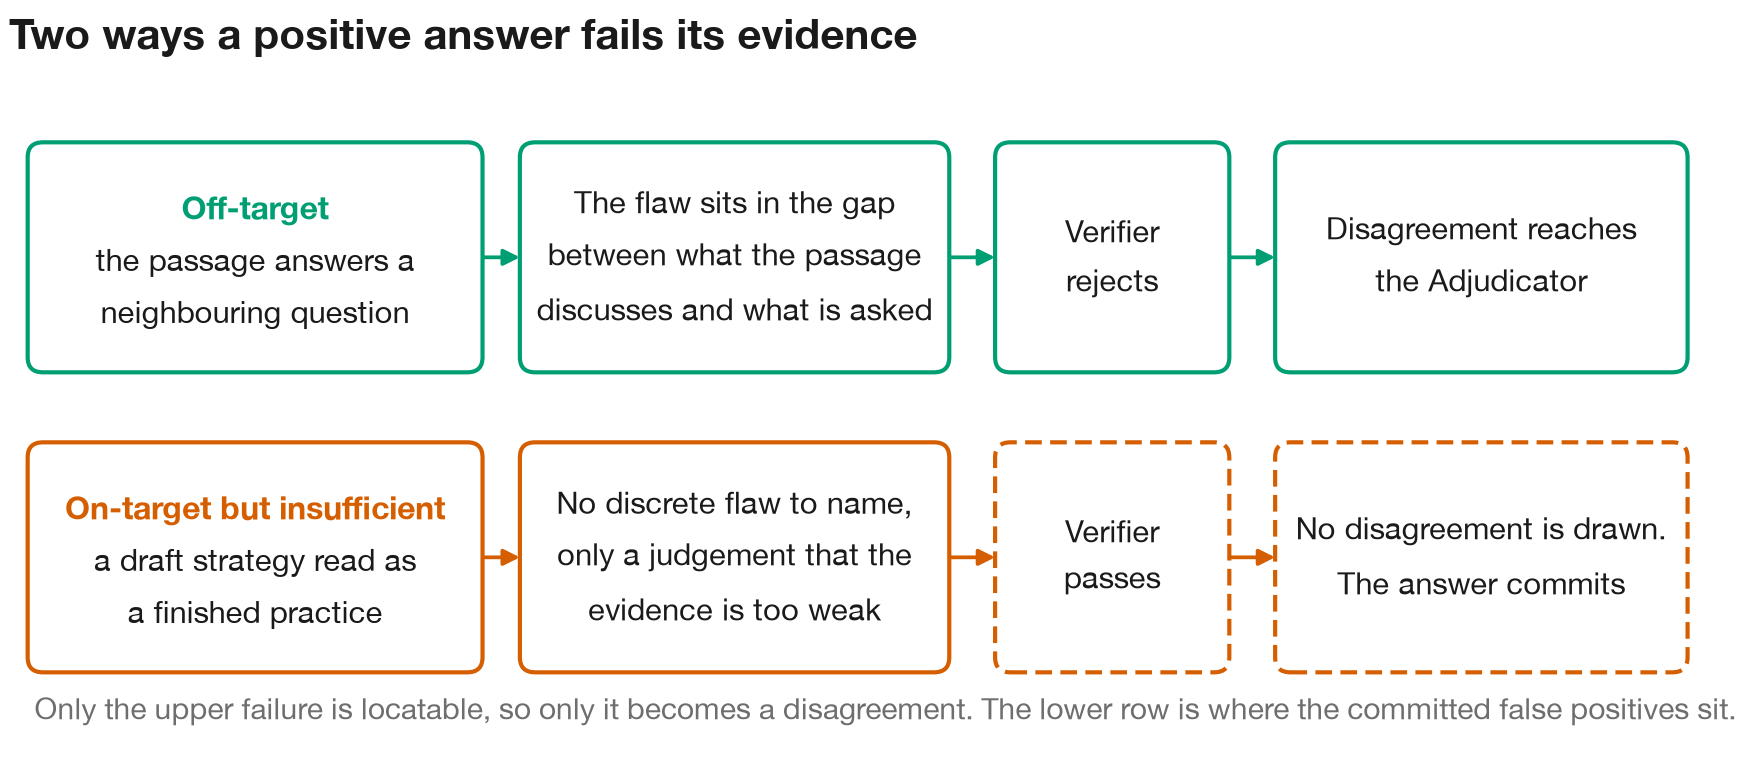
\includegraphics[width=5.9in,height=2.56287in]{media/media/image20.png}

@@CC@@Figure 5.2: Two ways a positive answer fails its evidence.@@/CC@@

The more consequential result is one none of these works anticipated. Cohen, Chowdhury and Zhu all study debate where the material to settle a claim is on hand and the open question~is how to reason over it, whereas the ODMI frequently offers evidence that is thin, adjacent or absent. The bottleneck this section has located, retrieval rather than the reasoning the debate was~built to sharpen, therefore falls outside what that literature was set up to examine, and it is where progression towards an automated assessor should be focused.

The Verifier is suited to an environment where it can set opposing evidence against the Researcher\textquotesingle s, where the answer turns on a reasoning difference over material both agents can see. The ODMI\textquotesingle s hard questions rarely provide that, since their evidence is thin, with adjacent material that reads as support for yes and nothing substantive that reads as support for no. There is little for two positions to be built from, so the debate has no practical opposition to stage. This is the setting the adversarial stance was meant for, since refuting over-reach on thin evidence is its stated purpose, yet it is the setting where it can do least. To refute a claim resting on weak but on-topic evidence the Verifier would need counterevidence the web does not hold, and without it the objection reduces to judging the evidence insufficient, a call it makes no more convincingly than the Researcher. The swarm\textquotesingle s contribution is therefore coverage, and the adversarial stance adds nothing beyond what a corroborative check already supplies.

\section{Reformulating the ODMI}\label{reformulating-the-odmi}

In their similar work, Fumega and Gao (2026) concluded that their approach still required human oversight rather than being fully autonomous. The results here extend that conclusion, since they show oversight does not have to fall evenly, as @@CC@@Figure 5.3 makes plain@@/CC@@. So, the useful question is which parts of the assessment the system can be trusted with and which have to stay manual.

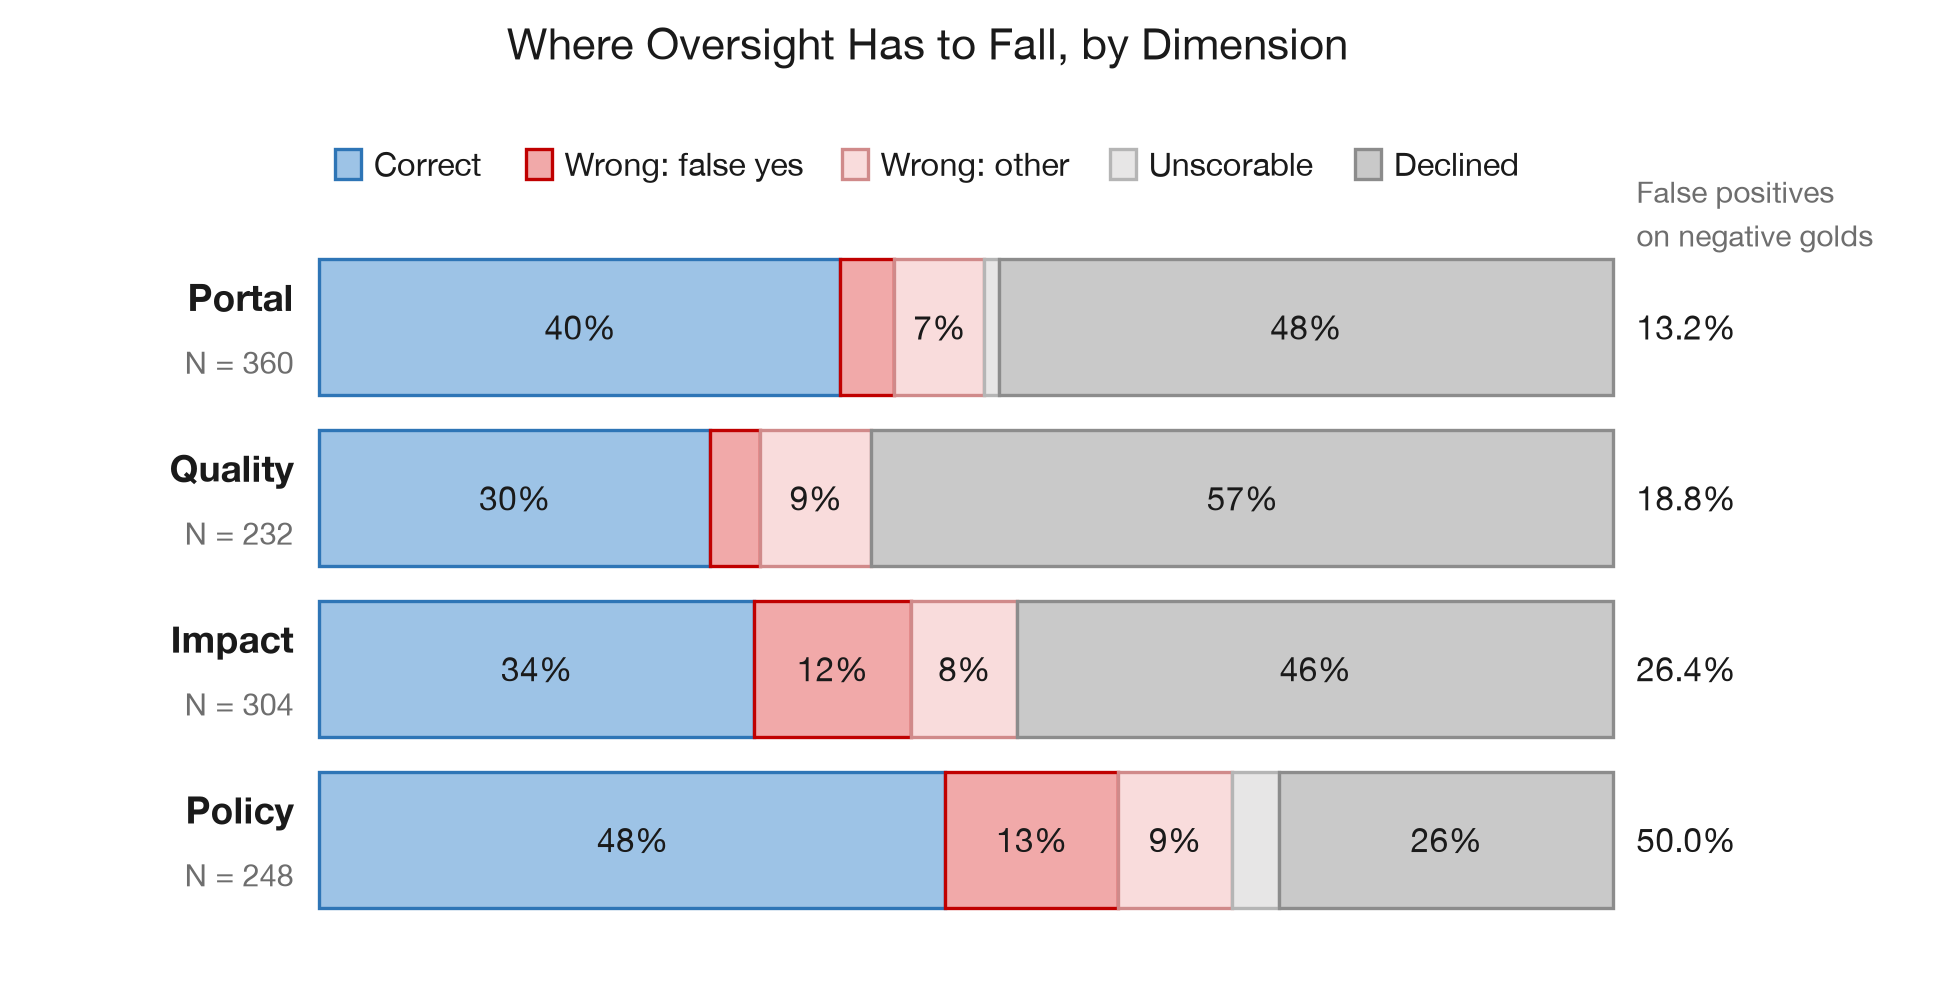
\includegraphics[width=5.89873in,height=3.01865in]{media/media/image21.png}

@@CC@@Figure 5.3: Outcome composition by ODMI dimension over the 1,144 evaluation pairs, ordered by false-positive rate on negative golds.@@/CC@@

The system is most reliable on the questions whose evidence is clear and whose nonexistence can be proved, and those are concentrated in the Portal dimension. Portal asks whether a feature is present on the national portal, which is visible on the page or absent from it, and the system commits on these at 0.784 accuracy with the lowest false-positive rate of the four dimensions. Quality behaves similarly on the questions it will answer, committing at 0.803 once its computable catalogue questions are set aside, with the second-lowest false-positive rate, though it is more cautious than Portal and declines more than half of what it is asked. Together the two are 74 of the 143 questions, the observable half of the questionnaire, the part that asks what a portal shows or a catalogue holds rather than what a team does behind it.

The catalogue questions make the case stronger still, since there the machine does not merely match the human process but appears to better it. §4.1 found the computed figure disagreeing with the recorded self-report on 44\% of the cells it could reach. The human process fills these by self-report and amends only a tenth of what countries submit, so a mechanical recount is the more trustworthy instrument on the very questions the human process is least equipped to check.

Where the process should still lie with the humans is Policy and Impact. Policy commits most readily and returns a wrong positive on half its negative questions, and the internal-practice questions spread across every dimension have little public evidence to retrieve, so both rest on internal knowledge and self-reporting that a human marker holds and the system cannot reach. These are the two operational dimensions, and leaving them to people plays to the one advantage the human process has.

The assessors meet the same limit. Across the thirty-six countries one Impact answer in eleven is "I don\textquotesingle t know", against none at all in Policy and Portal. The national teams cannot answer the dimension the swarm handles worst, so the evidence is missing for both parties. Jacobs and Wallach (2021) set out how assessments like the ODMI can diverge from what they mean to measure. They describe how there is a difference between the intangible construct, the openness of a nation's data in this case, and the tangible operationalisation, the ODMI assessment. The 143 questions stand in for that construct and approximate openness. §2.1 anticipated the shortfall, noting that automation poses a question to the assessment as much as the assessment poses one to the automation. This section takes that question up. How could the ODMI be best operationalised for a web-agent to be able to assess openness?

The reformulation this points to is not a matter of making the questions easier for a machine; it is a matter of aligning the operationalisation with the construct. A question that asks whether a team performs a practice, and accepts the team\textquotesingle s word, measures the claim about openness rather than openness itself. A question that asks for the published output of using that practice, rather than simply the existence of the practice itself, may measure openness more directly. The target of monitoring search keywords can be easily met, for example by saving a list of last month\textquotesingle s most frequent keyword terms. But setting the target of publishing the analysis of those keywords, what the team learnt from it and what they are acting on because of them, assesses the team\textquotesingle s engagement with the subject matter.

This is also the answer to the manipulation problem raised by Powers et al. (2002) and their work on automated essay scoring, where they found writers inflated an automated score more easily than they improved the actual work that was behind the score. An assessment is gameable when creating the evidence it rewards is cheaper than actually doing the activity the evidence is meant to prove@@CC@@, and the current questionnaire offers little resistance, since evidence of internal practices is largely unverifiable. @@/CC@@Requiring the published artefact reverses that for an openness index, and the current questions show the difference plainly. A country can claim to monitor its search terms at no cost, as PT28 invites, but it cannot fake having its portal\textquotesingle s source code public on GitHub, which PT43 asks for, nor a catalogue the quality assessment reads as machine-readable, which Q27 scores, without actually holding them. Where the cheapest way to satisfy a question is to produce the artefact, and the artefact is the open behaviour the question was after, scoring well on the assessment becomes a better approximation of the assessed quality.

{\def\LTcaptype{none} % do not increment counter
\begin{longtable}[]{@{}
  >{\raggedright\arraybackslash}p{(\linewidth - 6\tabcolsep) * \real{0.2836}}
  >{\raggedright\arraybackslash}p{(\linewidth - 6\tabcolsep) * \real{0.2321}}
  >{\raggedright\arraybackslash}p{(\linewidth - 6\tabcolsep) * \real{0.3116}}
  >{\raggedright\arraybackslash}p{(\linewidth - 6\tabcolsep) * \real{0.1727}}@{}}
\toprule\noalign{}
\begin{minipage}[b]{\linewidth}\raggedright
\textbf{@@CC@@Question group@@/CC@@}
\end{minipage} & \begin{minipage}[b]{\linewidth}\raggedright
\textbf{@@CC@@What it asks now@@/CC@@}
\end{minipage} & \begin{minipage}[b]{\linewidth}\raggedright
\textbf{@@CC@@What the reformed question would ask@@/CC@@}
\end{minipage} & \begin{minipage}[b]{\linewidth}\raggedright
\textbf{@@CC@@The source of evidence@@/CC@@}
\end{minipage} \\
\midrule\noalign{}
\endhead
\bottomrule\noalign{}
\endlastfoot
@@CC@@Portal features and data provision, 31 of 45@@/CC@@ & @@CC@@Whether a feature is present, with the URL already required@@/CC@@ & @@CC@@No change. Already answerable from outside@@/CC@@ & @@CC@@The live page@@/CC@@ \\
@@CC@@Portal usage and sustainability, 14 of 45@@/CC@@ & @@CC@@Whether the team monitors traffic or runs analytics@@/CC@@ & @@CC@@The published output of the monitoring, and what was acted on@@/CC@@ & @@CC@@The published report@@/CC@@ \\
@@CC@@Quality, computable from the catalogue, 9 of 29 (Q12, Q13, Q16 to Q18, Q21, Q22, Q25, Q27)@@/CC@@ & @@CC@@The team to select a percentage or count band for its own portal@@/CC@@ & @@CC@@No change to the question. Compute the figure from the harvested catalogue rather than accept the band@@/CC@@ & @@CC@@The catalogue itself@@/CC@@ \\
@@CC@@Quality, verifiable on the portal, 5 of 29 (Q5, Q8, Q11, Q15, Q19)@@/CC@@ & @@CC@@Whether a tag, standard, guideline or published page exists@@/CC@@ & @@CC@@No change. Q8 already requires the URL of the published page@@/CC@@ & @@CC@@The page, or the metadata@@/CC@@ \\
@@CC@@Quality, taken on the team\textquotesingle s word, 11 of 29 (Q1, Q3, Q4, Q6, Q7, Q9, Q10, Q14, Q20, Q23, Q24)@@/CC@@ & @@CC@@Whether the team monitors, investigates, undertakes efforts or uses a model@@/CC@@ & @@CC@@The published output of the practice: the monitoring report, the causes found, the deployment assessment@@/CC@@ & @@CC@@The published document@@/CC@@ \\
@@CC@@Policy framework, 13 of 31 (P1 to P12)@@/CC@@ & @@CC@@Whether a strategy or law contains a provision@@/CC@@ & @@CC@@Name the provision, and require the answer to quote it@@/CC@@ & @@CC@@The named clause@@/CC@@ \\
@@CC@@Policy governance, 9 of 31 (P13 to P21)@@/CC@@ & @@CC@@Whether a structure or an initiative exists@@/CC@@ & @@CC@@The share of local bodies that publish to the national portal@@/CC@@ & @@CC@@The portal\textquotesingle s publisher list@@/CC@@ \\
@@CC@@Policy implementation, 9 of 31 (P22 to P29)@@/CC@@ & @@CC@@Whether the team carries out a practice, as P28 asks for search-term monitoring@@/CC@@ & @@CC@@The published output of the practice@@/CC@@ & @@CC@@The published analysis@@/CC@@ \\
@@CC@@Impact, measuring reuse and awareness, 18 of 38@@/CC@@ & @@CC@@Whether the team measures reuse or runs awareness activities@@/CC@@ & @@CC@@The published measurement@@/CC@@ & @@CC@@The published report@@/CC@@ \\
@@CC@@Impact, reuse cases, 20 of 38@@/CC@@ & @@CC@@For a documented reuse case across four benefit areas@@/CC@@ & @@CC@@Inbound links and citations to datasets, repositories calling the portal API, dataset references in research and in the press@@/CC@@ & @@CC@@Third-party sites, outside the government estate@@/CC@@ \\
\end{longtable}
}

@@CC@@Table 5.2: What each group of questions would have to ask instead.

The demand that Policy framework questions@@/CC@@@@CL@@ in Table 5.2@@/CL@@@@CC@@ name their provision follows from @@/CC@@@@CL@@§4.5@@/CL@@@@CC@@, where the failure was over-reading an adjacent document rather than missing evidence. The governance rows ask for an outcome instead because a bare existence test is met by a nominal committee as easily as by a working one, and the monitoring rows, which run across all four dimensions, are where the reformulation is strongest.@@/CC@@

Impact resists reform more than the previous dimensions. The evidence lives outside the government websites, with an agent searching for work done by a third party that uses national data. This could live anywhere on the internet and carries no obligation to name the dataset it was built on. Dataset references in academic work and press or media use each leaves a public trace outside the government domain, and these are the least gameable evidence across the dimensions. The reformulated Impact dimension would be an independent, externally verifiable assessment of the demand side of openness.

Openness that a government enacts, whether a policy adopted, a portal feature deployed, a standard met or an analysis published, leaves a public trace, and any dimension built on it can be assessed from the outside once the question demands the trace rather than the claim. Impact leaves its trace on the sites of the people who used the data, so what it calls for is a different retrieval design as well as a different question, one that searches outward from the portal instead of inward across a government estate. All four dimensions could therefore be delegated under a reformed questionnaire. Holding the assessment to public evidence divides the questionnaire into the questions that can be externally verified and the questions taken on self-reported claims. Closing that division would not only improve the possibility of automation but would also close the gap between the construct and operationalisation of openness, because a country that publishes the analysis, the register or the conformant catalogue has demonstrated openness in the act of producing the evidence.

This is the answer to RQ3. Responsibility is not handed over whole or withheld whole but split by type of question, the machine taking what the public record can answer, and the human keeping what needs internal knowledge.@@CC@@ The observable half is the part the machine can take. In its current form, the swarm commits to about half of these questions, so a quarter of the whole questionnaire outright. It can flag the observable questions it cannot commit to, and leave the operational half wholly to the human.@@/CC@@

\section{Threats to Validity}\label{threats-to-validity}

@@CC@@Appendix A holds the full register of thirty-four modes by which the swarm can commit a wrong answer, twenty-two of them structural. The threats set out below are those bearing on the reported figures.@@/CC@@

Every retrieval finding is conditional on a single search stack. The system runs Serper and trafilatura for every query, and although the DIY pipeline laid out in §3.3 performed at least as well as the two commercial APIs it replaced, Tavily and Brave (see Experiments appendix), one implementation cannot rule out a systematic blind spot in what this combination returns. The conclusion of §5.2 is the finding most exposed to it, since holding that the binding constraint is retrieval assumes the evidence is scarce rather than that this pipeline failed to surface it.

@@CC@@Several figures rest on samples too small to estimate what they describe with precision. The replicate battery of §4.6 holds 148 pairs and the evaluation set eight countries, so confidence intervals on accuracy are wide. The ablation of §4.7 is not among them, since it runs the four arms over all 1,144 evaluation pairs and returns an equivalence on the Verifier\textquotesingle s stance at p below 0.0001, which establishes the absence of a difference instead of failing to find one. The constraint is partly the compute and search throughput available at this scale, and partly the ODMI itself, which contains thirty-six countries in total.@@/CC@@

External validity is bounded by how the evaluation set was built. Eight of the thirty-six countries were chosen to span language resource and negative-gold share rather than sampled at random, which over-represents low-resource languages and negative-rich questionnaires by design@@CC@@, a gap the always-yes baseline makes concrete at 59.4\% on these eight against 81.8\% across all thirty-six@@/CC@@, so the pooled figures do not describe the remaining twenty-eight. The extrapolation to roughly 200 hours and £1,700 for a full cycle assumes those countries behave like these eight, and the reconstructed ranking is correlated over a maturity range far wider than a real cohort spans, which makes an ordering easier to preserve than it would be across countries separated by a point or two.

The comparator is also a year out of date. The key records the 2025 cycle while the swarm read the web in 2026, so a country that adopted a policy or shipped a portal feature in the intervening year is marked wrong for answering ``yes'', and an unknown share of the committed false positives may be the swarm describing a later state of the world correctly. Testing against the 2026 key, unreleased at the time of writing, could raise the raw match rate if the average maturity continues to climb \textbf{@@CC@@as §1.2 records@@/CC@@} it doing each cycle, as there are more questions answered ``yes'' across the countries, which the system performs better on. However, the always-yes baseline would rise with it, so a higher score would not by itself show the system had improved.\textbf{@@CC@@ @@/CC@@}

Construct validity is threatened by the non-independence of the deterministic catalogue recompute, which carries the argument that the answer key cannot be fully trusted. The figures come from a single snapshot of the harvested datasets, and the Verifier repeats the same arithmetic over the same cached harvest without reaching a second source, so a divergence from the key cannot establish which of the two figures describes the portal. The one independent computation of these metrics is published by the Metadata Quality Assessment on data.europa.eu, which the leakage controls deny-list because that domain also publishes the answer key.

The language confound in @@CL@@§4.4@@/CL@@ was not resolved directly. To determine whether the higher abstention in the lower-resource stratum reflects the model's poorer reading of those languages, or simply fewer publications to read, we would need to rerun the same pairs on translated evidence, keeping the evidence constant while varying only the language the model reads. Conducting that experiment across the stratum required translation volume beyond the free tiers, so a comparison at a useful scale was not possible. Consequently, the decomposition in @@CL@@§4.4@@/CL@@ identifies the gap in the Researcher's confidence rather than in the Verifier's judgement, leaving the second branch of the question the stratification was meant to address unresolved.

\section{Legal, Social, Ethical and Professional Issues}\label{legal-social-ethical-and-professional-issues}

There are two requirements of the BCS Code of Conduct and the IET Rules of Conduct that bear directly on this work: The duty to act in the public interest and the duty to work within the limits of demonstrated competence. The first of these governs how the system collects its evidence. Every request identifies the project, the institution and a contact address. The retrieval layer reads each portal\textquotesingle s robots.txt before fetching and refuses any path the portal excludes, and where a site presents an automated challenge the fetch waits within a fixed budget and then abandons the page, so no attempt is made to defeat the check. A separate set of controls, described in §3.6, keeps the evaluation from reading ODMI\textquotesingle s own published answers. The questionnaire and the published answers it is measured against are Commission documents, reusable under Decision 2011/833/EU and released on data.europa.eu under a Creative Commons Attribution licence, so their use here carries an attribution requirement and nothing further. Evidence drawn from national portals is quoted in short passages from public pages, with the source URL recorded alongside each quotation. Model access runs through a local proxy onto a flat-rate subscription, so the costs reported in §4.8 are arithmetic equivalents computed from published per-token rates, and no figure in this report is billed spend.

§5.3 answers the second requirement, in that a system which commits to answers it cannot evidence would be worse than no system at all, and the boundary between the questions the system can be trusted with and those it cannot therefore matters more than the aggregate accuracy. What this work supports is the narrow claim that an identified subset of the assessment can be automated under stated conditions, with the remainder left to the people who carry it out now.
